\documentclass[conference]{IEEEtran}
% \IEEEoverridecommandlockouts
% The preceding line is only needed to identify funding in the first footnote. If that is unneeded, please comment it out.
\usepackage{cite}
\usepackage{amsmath,amssymb,amsfonts}
\usepackage{algorithmic}
\usepackage{graphicx}
\usepackage{textcomp}
\usepackage{xcolor}
\usepackage{caption}
\def\BibTeX{{\rm B\kern-.05em{\sc i\kern-.025em b}\kern-.08em
    T\kern-.1667em\lower.7ex\hbox{E}\kern-.125emX}}
\begin{document}

\bibliographystyle{IEEEtran}

\title{Applying ResNet and Inception Module Techniques for Skin Cancer Classification on Breast Histopathology Images Dataset with Convolutional Neural Networks\\
}

\author{\IEEEauthorblockN{1\textsuperscript{st} Pedro Almeida}
\IEEEauthorblockA{\textit{Department of Ocean \& Mechanical Engineering} \\
\textit{Florida Atlantic University}\\
Boca Raton, United States \\
palmeida2016@fau.edu}
}

\maketitle

\begin{abstract}

\end{abstract}

\begin{IEEEkeywords}
artificial neural network, machine learning, convolutional neural network
\end{IEEEkeywords}

\section{Introduction}
Over the past 40 years \cite{Fukushima1980}, the field of object detection in machine learning has made massive strides in classification and detection capabilities. In addition to the expected improvements stemming from larger datasets, deeper models, and more powerful machines, much of the advancement owes to new and improved network architectures and novel algorithms. These techniques, often designed with specific datasets in mind, take advantage of the structure of the data to optimize the amount of information extracted per layer. The difficulty in designing the networks stem from the increasingly numerous design choices in determining hyper-parameters (the number of channels in a layer , filter sizes, strides, pooling layer parameters, dropout rates, \emph{etc.}) and the large selection of techniques in constructing the network architecture \cite{Krizhevsky2012, Szegedy2014, He2016, Huang2016, Simonyan2014, Hu2017, Xie2017, huang2019convolutional, Zhao2021}.

The family of inception models \cite{Szegedy2014, Szegedy2015, Szegedy2016} tackled the problem by introducing an extra dimension cardinality: the number of independent paths within a layer. The central method employed involves splitting the input of a layer into lower-dimensional embeddings whereby each is transformed by a set of specialized filters with different kernel sizes, which are then concatenated. The \emph{split-transform-merge} method has been shown to approximate the representational power of large, dense layers, but at a substantially lower computational complexity. Despite showing good improvements in accuracy, the inception module suffers from a difficulty in tailoring filter numbers and sizes for different datasets/objectives; although the right combination can yield significant improvements to the accuracy, it is generally unclear as to how to adapt the Inception module architecture of a given problem, especially in combination with other complex transformations and hyper-parameters are involved.

Another strategy introduced by the family of ResNet models and its variants proposes the use of residual learning through stacking modules of the same topology. This simple rule creates a an effective strategy for constructing very deep network architectures that are applicable to a wide range of tasks, owing partially to the reduction of free choices for hyper-parameters.

The objective of the report is to explore the combination of some of these techniques \cite{Szegedy2014, He2016} through the Breast Histopathology Dataset \cite{Mooney2017}. The dataset contains 162 whole mount slide images of a breast cancer variant called Invasive Ductal Carcinoma scanned at forty-times magnification. As of 2019, breast cancer affects 1 in 8 \cite{DeSantis2019} women during their lifetime, registering roughly 268,600 new cases every year. Invasive Ductal Carcinoma, also known as Infiltrating Ductal Carcinoma, is the most common type breast cancer, accounting for 80\% \cite{Sharma2010} of breast cancer diagnoses. As is the case for most cancers, early detection accounts for most of successful treatments of the disease; as the cancer progresses to the later stages, the odds of spreading to nearby organs increases \cite{Milosevic2018}, thus furthering the risk of the death of the patient.

We propose a Convolutional Neural Network architecture 

\section{Related Work}
Prior to the introduction of Convolutional Neural Networks, the identification of malignant and benign regions in histopathology images largely relied on detection of histologic primitives -- markings for detection of breast cancer in histopathology images -- and feature extraction to characterize regions \cite{Doyle2008,Dundar2011,Niwas2011,Basavanhally2013}. In Doyle \emph{et al.} 2008 \cite{Doyle2008} the proliferation of nuclei is analyzed by detecting textural and graph features of histopathological data to determine the discriminating characteristics of tissue patterns in 3 different window sizes. Dundar \emph{et al.} 2011 \cite{Dundar2011} applies feature analysis of the perimeter for cell size, the ratio of major to minor axis in the best fitting ellipse for cell shape, and mean of the gray-level intensity for nucleoli appearance to train a Multiple Instance Learning (MIL) model to distinguish between positive and negative samples. In Niwas \emph{et al.} 2011 \cite{Niwas2011} the texture features of nuclei in biopsy images extracted using Log-Gabor Wavelets are used to classify breast carcinomas. In Basavanhally \emph{et al.} 2013 \cite{Basavanhally2013} the histopathology slides are converted into a new color space and processed with color-gradient based geodesic active contour to segment nuclear regions.

Though the techniques described provided massive improvements to the manual analysis previously performed by pathologists, they rely heavily on the post-processing of images rather than computer vision. The result is a prediction model with a lesser understanding of the image structure and spatial positioning of features, which often leads to lower accuracy in predicitons. As such, the latest proposed solutions to the classification of breast cancer histopathology slides have applied Deep Convolutional Neural Networks and novel methods \cite{Dabeer2019,Mahmood2020,Gour2020,Wahab2020,Zainudin2020}. In Dabeer \emph{et al.} 2019 \cite{Dabeer2019} the histopathological slides are used to train a standard convolutional neural network with blocks constituting of a convolutional layer followed by a pooling layer to achieve an accuracy of 93.45\% on the BreakHis database.

Since the introduction of Convolutional Neural Networks (CNN), the model architecture off CNNs has remained largely static: a series of convolutional layers followed by optional normalization and pooling layers and finally one or more dense layers reducing to the output. This standard architecture and its variations have reigned dominant in accurately classifying objects in small and large datasets alike, from MNIST, CIFAR, ImageNet, MS-COCO, SVHN, and others. For larger datasets especially, the latest novel idea has been the introduction of deeper networks with dropout layers to correct for overfitting.

The tradeoff for adding more layers to a network is apparent in the time to train; as the model grows in size and increases the number of weights, the backwards propagation in updating the weights takes progressively longer, thus greatly adding to the required time to train. Furthermore, although the development of newer, more powerful machines and better parallelization and multi-processing techniques can somewhat mitigate the additional computational cost.

\section{Methods}
\subsection{ResNet Layer}
The first CNN modification applied in the model architecture employs residual learning within the convolution layers. As described by He \textit{et al.} \cite{He2016}, let us consider a residual layer within a neural network defined as:

\begin{equation}
y = \mathcal{F} \left(x_i,\{W_i\}\right) + x
\label{residual_layer_equation}
\end{equation}

In Eq. \ref{residual_layer_equation}, $x$ and $y$ are the input and output vectors of the layer respectively. The function $\mathcal{F} \left(x_i,\{W_i\}\right)$ represents the mapping of inputs to outputs given a set of weights $W_i$ for each of the feature maps of the inner convolutions \cite{He2016}. For the example shown in Fig.~\ref{ResNet_Layer_Model}, the input $x$ to the layer passes through 4 convolutional layers, which together constitute $\mathcal{F}(x)$ before the concatenation with the input $x$. The final concatenation of the output of the feature maps and initial input is a element-wise addition performed channel by channel, which is then passed through an activation layer. In the original paper by He, the residual function $\mathcal{F} \left(x_i,\{W_i\}\right)$ constitutes of 2-3 fully connected layers \cite{He2016}. The proposed architecture slightly alters the core ResNet model by substituting the fully connected layers by convolutional layers followed by Rectified Linear Unit -- also known as ReLU -- activation functions.

The proposed architecture implements the ResNet layers as proposed by He \emph{et al.} with an exponentially increasing number of filters in subsequent layers (32, 64, 128, 256). Each of the convolutions is followed by ReLU activation units.

\begin{figure}
\centering
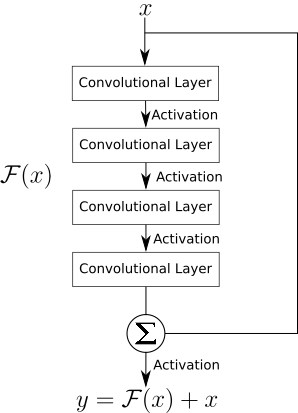
\includegraphics[width=0.3\textwidth]{figures/ResNet_Model.png}
\caption{Model of ResNet Layer with 4 Convolutions.}
\label{ResNet_Layer_Model}
\end{figure}

\subsection{Inception Module Layer}
The second CNN modification applied in the network architecture is the use of the Inception Module \cite{Szegedy2014} designed by Szegedy \emph{et al.} Unlike the ResNet Layer, the inception module bypasses the deepening of neural networks for better performance through optimal local sparse structures. The structure of the module is founded on the parallelization of inputs into paths with convolutional layers of different kernel sizes.

In layers closer to the input image, one can expect the output of convolutional filters to concentrate in local regions, which could be covered by a layer of 1x1 convolutions in the next layer. However, over larger patches, the outputs of the convolutions will lead to fewer, more spread out clusters that cannot be easily covered by convoultuions. As such, in order to avoid the patch-alignment issues, Szegedy \emph{et al.} proposes restricting the kernel size to 1$\times$1, 3$\times$3, and 5$\times$5. The final addition to the inception module is the addition of 1$\times$1 convolutions before the larger kernel size convolutional layers. The reason behind the choice is that, especially in the originally proposed architecture where inception modules are stacked to create the network, the numbre of 5$\times$5 convolutions can be prohibitely expensive. As such, the merging of output layers in the module would inevitably lead to exponential growth, thus adding immense computational complexity to the model. The proposed 1$\times$1 convolutions before the 3$\times$3 and 5$\times$5 would compute the reductions, thus preveting that growth. 

\begin{figure}
\centering
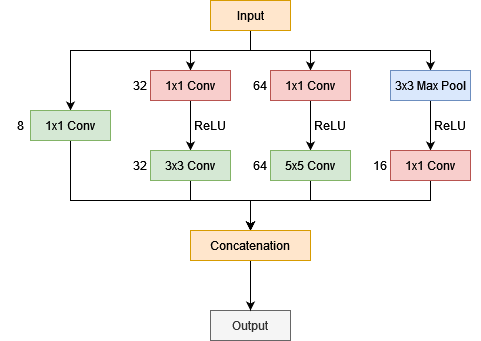
\includegraphics[width=0.4\textwidth]{figures/Inception_Model.png}
\caption{Model of Inception Layer with 4 parallel paths.}
\label{Inception_Model}
\end{figure}

The proposed architecture implements the Inception Module layers as proposed by Szegedy {et al.} with 8, 32, 64, and 16 filters as shown in Fig. \ref{Inception_Model}. 

\subsection{Network Architecture}
\subsection{Dataset and Data Augmentation}
The dataset consists of the data compiled by Cruz-Roa \emph{et al.} in 2014 \cite{Cruz-Roa2014}. The was collected during visual analysis of tissue slides stained with hematoxylin and eosin (H\&E) by pathologists. The dataset contains the sampling images of 162 different patieents identified by professionals as either benign or malignant. Each of the 162 samples in the dataset have been partitioned to create 277,524 50x50-pixel patches, of which 198,738 are IDC negative and 78,786 are IDC positive. In preparation for the training cycle, the samples were shuffled and distributed into training, validation, and testing sets constituting 60\%, 20\%, and 20\% of the total number respectively. To account for the imbalance in negative and positive samples, the distribution  ensures the ratio of negative to positive samples is consistent across all three sections of the dataset.

\begin{figure}
\centering
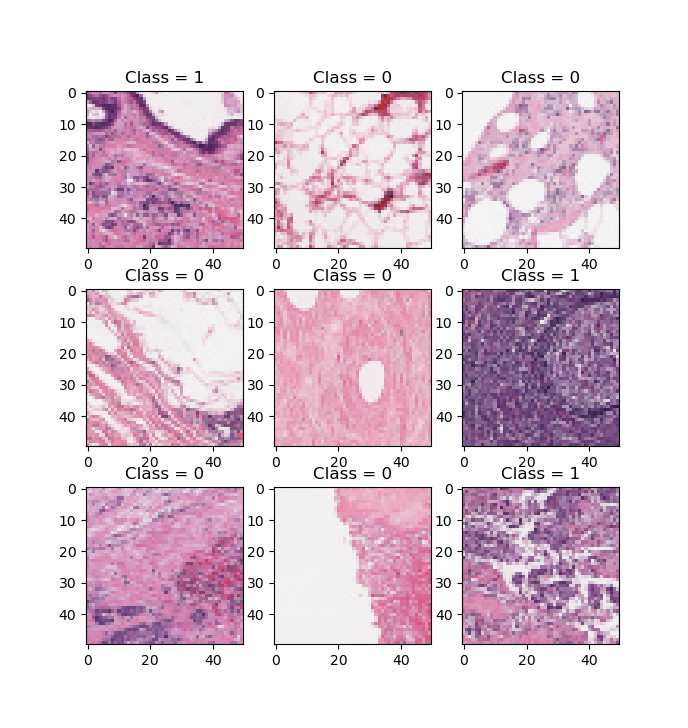
\includegraphics[width=0.4\textwidth]{figures/dataset_example.png}
\caption{Example of partitioned images found in dataset.}
\label{dataset_example}
\end{figure}

The images in each of the sections is then converted from to RGB for training with each color channel zero-centered. Since the spatial orientation and location of the features in the image is not relevant to the classification, the data loader for the model will randomly shuffle the images and choose wether to reflect the image horizontally, vertically, or any combination for each of the epochs, thus providing more variation to the dataset and hopefully generalizing the model.

\subsection{Training the Network}
 The training of the model applies two important callbacks to maximize the efficiency of the model to converge to the lowest loss. The first of the methods applied is an adaptive learning rate as given in the Keras machine learning library. Using the built-in function \emph{ReduceLROnPlateau}, the model will monitor the change in validation loss between epochs and automatically reduce the learning rate by a factor of 10 if the change in validation loss is lower than the threshold \emph{min\_delta} (given as 0.0001) for 3 consecutive epochs. The second callback serves to prevent the model from continuing training if its validation loss does not decrease for 10 consecutive epochs, which is implemented with the Keras \emph{EarlyStopping} class.

The CNN was trained over the course of 3 hours on a RTX-2070 GPU as shown in Fig. \ref{training_accuracy} and \ref{training_loss}.

\begin{figure}
\centering
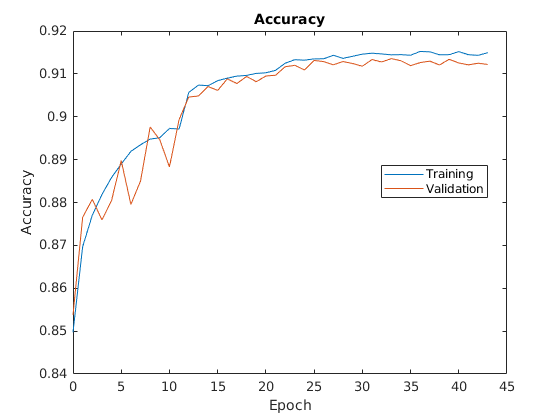
\includegraphics[width=0.4\textwidth]{figures/training_accuracy.png}
\caption{Plot of training accuracy on train and validation data.}
\label{training_accuracy}
\end{figure}

\begin{figure}
\centering
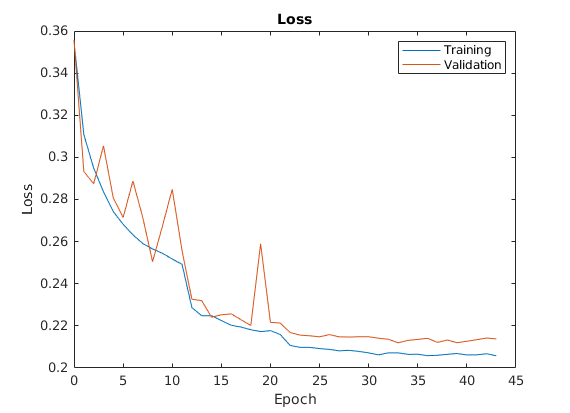
\includegraphics[width=0.4\textwidth]{figures/training_loss.png}
\caption{Plot of training loss on train and validation data.}
\label{training_loss}
\end{figure}

\section{Results}

\section{Analysis and Discussion}

\section{Conclusions}

\section*{Acknowledgment}
The author would like to thank Dr. Xingquan Zhu for valuable discussions and recommendations in writing this paper.

\bibliography{citations}

\end{document}
